
% Spellcheck: ok
% Mikes: ok

\chapter{What You Really Need to Know About Classical Statistics}{}{}
\label{ch:statistics}

\index{data analysis!statistics|(} 
\index{statistics|(} 

\Fint{Basic classical statistics has always been somewhat of a mystery to
me: a topic full of obscure} notions, such as $t$-tests and $p$-values,
and confusing statements like ``we fail to reject the null
hypothesis''---which I can read several times and still not know 
if it is saying yes, no, or maybe.\footnote{I am not alone---even
  professional statisticians have the same experience.  See, for
  example, the preface of \cit{Bayesian Statistics}{Peter M.\
    Lee}{Hodder \& Arnold}{2004}} To top it all off, all this
formidable machinery is then used to draw conclusions that don't seem
to be all that interesting---it's usually something about whether
the means of two data sets are the same or different. Why would I
care?

Eventually I figured it out, and I also figured out why the field
seemed so obscure initially. In this chapter, I want to explain what
classical statistics does, why it is the way it is, and what it is
good for. This chapter does not attempt to teach you how to perform
any of the typical statistical methods: this would require a separate
book. (I will make some recommendations for further reading on this
topic at the end of this chapter.) Instead, in this chapter I will
tell you what all these other books \emph{omit}.

Let me take you on a trip. I hope you know where your towel is.

% ============================================================
\section{Genesis}

\index{statistics!historical development} 

To understand classical statistics, it is necessary to realize how it
came about. The basic statistical methods that we know today were
developed in the late 19th and early 20th centuries, mostly in Great
Britain,\vadjust{\pagebreak} by a very small group of people. Of those, one worked for the
Guinness brewing company and another---the most influential one of
them---worked at an agricultural research lab (trying to increase crop
yields and the like). This bit of historical context tells us
something about their working conditions and primary challenges.

\begin{unnumlist}
\subparagraph{No computational capabilities}
\item All computations had to be
  performed with paper and pencil.
      
\subparagraph{No graphing capabilities, either}
\item All graphs had to be
  generated with pencil, paper, and a ruler. (And complicated
  graphs---such as those requiring prior transformations or
  calculations using the data---were especially cumbersome.)

\subparagraph{Very small and very expensive data sets}      
\item Data sets were small
  (often not more than four to five points) and could be obtained only
  with great difficulty. (When it always takes a full growing season
  to generate a new data set, you try \emph{very} hard to make do with
  the data you already have!)
\end{unnumlist}

In other words, their situation was almost entirely the opposite of
our situation today:

\begin{itemize}
\item Computational power that is essentially free (within reason)
\item Interactive graphing and visualization capabilities on every
  desktop
\item Often huge amounts of data
\end{itemize}

It should therefore come as no surprise that the methods developed by
those early researchers seem so out of place to us: they spent a great
amount of effort and ingenuity solving problems we simply no longer
have!  This realization goes a long way toward explaining why
classical statistics is the way it is and why it often seems so
strange to us today.

By contrast, \emph{modern} statistics is very different. It places
greater emphasis on nonparametric methods and Bayesian reasoning, and
it leverages current computational capabilities through simulation and
resampling methods. The book by Larry Wasserman (see the recommended
reading at the end of this chapter) provides an overview of a more
contemporary point of view.

However, almost all \emph{introductory} statistics books---that is,
those books one is likely to pick up as a beginner---continue to limit
themselves to the same selection of slightly stale topics. Why is
that? I believe it is a combination of institutional inertia together
with the expectations of the ``end-user'' community.  Statistics has
always been a support science for other fields: originally agriculture
but also medicine, psychology, sociology, and others. And these
fields, which merely apply statistics but are not engaged in actively
developing it themselves, continue to operate largely using classical
methods.  However, the machine-learning community---with its roots in
computer science but great demand for statistical methods---provides a
welcome push for the widespread adoption of more modern methods.

Keep this historical perspective in mind as we take a closer look at
statistics in the rest of this chapter.
  
% ============================================================
\section{Statistics Defined}

\index{statistics!about|(}
 
All of statistics deals with the following scenario: we have a
\emph{population}---that is the set of all possible outcomes.
Typically, this set is large: all male U.S.\ citizens, for example, or
all possible web-server response times. Rather than dealing with the
total population (which might be impossible, infeasible, or merely
inconvenient), we instead work with a \emph{sample}. A sample is a
subset of the total population that is chosen so as to be
representative of the overall population. Now we may ask: what
conclusions about the overall \emph{population} can we draw given one
specific \emph{sample}? It is this particular question that classical
statistics answers via a process known as \emph{statistical
  inference}: properties of the population are inferred from
properties of a sample.

Intuitively, we do this kind of thing all the time. For example, given
the heights of five men (let's say 178 cm, 180 cm, 179 cm, 178 cm, and
180 cm), we are immediately comfortable calculating the average (which
is 179 cm) and concluding that the ``typical'' body size for all men
in the population (not just the five in the sample!) is 179 cm, ``more
or less.'' This is where formal classical statistics comes in: it
provides us with a way of making the vague ``more or less'' statement
precise and \emph{quantitative}. Given the sample, statistical
reasoning allows us to make specific statements about the population,
such as, ``We expect $x$ percent of men to be between $y$ and $z$ cm
tall,'' or, ``We expect fewer than $x$ percent of all men to be taller
than $y$ cm,'' and so on.

Classical statistics is mostly concerned with two procedures:
\emph{parameter estimation} (or ``estimation'' for short)\index{parameter estimation}\index{estimation, parameter estimation} and
\emph{hypothesis testing}.\index{hypothesis testing}\index{tests!hypothesis testing} Parameter estimation works as follows. We
assume that the population is described by some distribution---for
example, the Gaussian: 
%
\[
N(x;\mu,\sigma) = \frac{1}{\sqrt{2 \pi} \sigma}
  \exp \paren{ -\frac{1}{2} \paren{ \frac{x-\mu}{\sigma} }^2 }
\]
%
and we seek to estimate values for the parameters ($\mu$ and
$\sigma$ this case) from a sample. Note that once we have estimates
for the parameters, the distribution describing the population is
fully determined, and we can (at least in principle) calculate any
desired property of the population directly from that distribution.
Parameter estimation comes in two flavors: \emph{point estimation} and
\emph{interval estimation}.  The first just gives us a specific value
for the parameter, whereas the second gives us a range of values that
is supposed to contain the true value.

Compared with parameter estimation, hypothesis testing is the weirder
of the two procedures. It does not attempt to quantify the size of an
effect; it merely tries to determine whether there is any\vadjust{\pagebreak} effect at
all. Note well that this is a largely theoretical argument; from a
practical point of view, the existence of an effect cannot be
separated entirely from its size. We will come back to this point
later, but first let's understand how hypothesis testing works.

Suppose we have developed a new fertilizer but don't know yet whether
it actually works. Now we run an experiment: we divide a plot of land
in two and treat the crops on half of the plot with the new
fertilizer.  Finally, we compare the yields: are they different? The
specific amounts of the yield will almost surely differ, but is this
difference due to the treatment or is it merely a chance fluctuation?
Hypothesis testing helps us decide how large the difference needs to
be in order to be \emph{statistically significant}.

Formal hypothesis testing now proceeds as follows. First we set up the
two hypotheses between which we want to decide: the \emph{null
  hypothesis} \index{null hypotheses} (no effect; that is there is no difference between the two
experiments) and the \emph{alternate hypothesis} \index{alternate hypotheses} (there is an effect
so that the two experiments have significantly different outcomes). If
the difference between the outcomes of the two experiments is
statistically significant, then we have sufficient evidence to
``reject the null hypothesis,'' otherwise we ``fail to reject the null
hypothesis.'' In other words: if the outcomes are not sufficiently
different, then we retain the null hypothesis that there is no effect.

This convoluted, indirect line of reasoning is required because,
strictly speaking, no hypothesis can ever be proved correct by
empirical means. If we find evidence \emph{against} a~hypothesis, then
we can surely reject it. But if we \emph{don't} find evidence against
the hypothesis, then we retain the hypothesis---at least until we do
find evidence against it (which may possibly never happen, in which
case we retain the hypothesis indefinitely).

This, then, is the process by which hypothesis testing proceeds:
because we can never prove that a treatment was successful, we instead
invent a contradicting statement that we can prove to be \emph{false}.
The price we pay for this double negative (``it's \emph{not} true that
there is \emph{no} effect'') is that the test results mean exactly the
opposite from what they seem to be saying: ``retaining the null
hypothesis,'' which sounds like a success, means that the treatment
had no effect; whereas ``rejecting the null hypothesis'' means that
the treatment did work. This is the first problem with hypothesis
testing: it involves a convoluted, indirect line of reasoning and a
terminology that seems to be saying the exact opposite from what it
means.

But there is another problem with hypothesis testing:\index{statistical significance}\index{significance, statistical significance} it makes a
statement that has almost no practical meaning! In reducing the
outcome of an experiment to the Boolean choice between ``significant''
and ``not significant,'' it creates an artificial dichotomy that is
not an appropriate view of reality. Experimental outcomes are not
either strictly significant or strictly nonsignificant: they form a
continuum. In order to judge the results of an experiment, we need to
know where along the continuum the experimental outcome falls
\emph{and} how robust the estimate is. If we have this information, we
can decide how to interpret the experimental result and what
importance to attach to it.

Classical hypothesis testing exhibits two well-known traps. The first
is that an experimental outcome that is \emph{marginally} outside the
statistical significance level abruptly changes the interpretation of
the experiment from ``significant'' to ``not significant''---a
discontinuity in interpretation that is not borne out by the minimal
change in the actual outcome of the experiment.  The other problem is
that almost any effect, no matter how small, can be made
``significant'' by increasing the sample size.  This can lead to
``statistically significant'' results that nevertheless are too small
to be of any practical importance. All of this is compounded by the
arbitrariness of the chosen ``significance level'' (typically 5
percent). Why not 4.99 percent? Or 1 percent, or 0.1 percent?  This
seems to render the whole hypothesis testing machinery (at least as
generally practiced) fundamentally inconsistent: on the one hand, we
introduce an absolutely sharp cutoff into our interpretation of
reality; and on the other hand, we choose the position of this cutoff
in an arbitrary manner. This does not seem right.

(There is a third trap: at the 5 percent significance level, you can
expect 1 out of 20 tests to give the wrong result. This means that
if you run enough tests, you will always find one that supports
whatever conclusion you want to draw. This practice is known as
\emph{data dredging} and is strongly frowned upon.)

Moreover, in any practical situation, the actual size of the effect is
so much more important than its sheer existence. For this reason,
hypothesis testing often simply misses the point. A project I recently
worked on provides an example of this. The question arose as to
whether two events were statistically independent (this is a form of
hypothesis testing). But, for the decision that was ultimately made,
it did not matter whether the events truly were independent (they were
not) but that treating them as independent made no measurable
difference to the company's balance sheet.

Hypothesis testing has its place but typically in rather abstract or
theoretical situations where the mere existence of an effect
constitutes an important discovery (``Is this coin loaded?'' ``Are
people more likely to die a few days after their birthdays than
before?'').  If this describes your situation, then you will quite
naturally employ hypothesis tests. However, if the \emph{size} of an
effect is of interest to you, then you should feel free to ignore
tests altogether and instead work out an estimate of the
effect---including its confidence interval. This will give you the
information that you need. You are not ``doing it wrong'' just because
you haven't performed a significance test somewhere along the way.

Finally, I'd like to point out that the statistics community itself
has become uneasy with the emphasis that is placed on tests in some
fields (notably medicine but also social sciences). Historically,
hypothesis testing was invented to deal with sample sizes so small
(possibly containing only four or five events) that drawing any
conclusion at all was a challenge. In such cases, the broad
distinction between ``effect'' and ``no effect'' was about the best
one could do. If interval estimates are available, there is no reason
to use statistical tests. The Wikipedia entry on $p$-values (explained
below) provides some starting points to the controversy.

I have devoted quite a bit of space to a topic that may not seem
especially relevant. However, hypothesis tests feature so large in
introductory statistics books and courses and,~at the same time, are
so obscure and counterintuitive, that I found it important to provide
some background.  In the next section, we will take a more detailed
look at some of the concepts and terminology that you are likely to
find in introductory (or not-so-\break introductory) statistics books and
courses.
  
\index{statistics!about|)}

% ============================================================
\section{Statistics Explained}

\index{statistics!distributions|(}
\index{distributions!statistics|(}  

In Chapter \ref{ch:probability}, we already encountered several
well-known probability distributions, including the binomial (used for
trials resulting in Success or Failure), the Poisson (applicable in
situations where events are evenly distributed according to some
density), and the ubiquitous Normal, or Gaussian, distribution. All of these distributions describe real-world, 
observable phenomena.

In addition, classical statistics uses several distributions that
describe the distribution of certain quantities that are not observed
but calculated. These distributions are not (or not usually) used to
describe events in the real world. Instead, they describe how the
outcomes of specific typical calculations involving random quantities
will be distributed. There are four of these distributions, and they
are known as \emph{sampling distributions}. \index{sampling distributions} \index{distributions!sampling distributions} 

The first of these (and the only one having much use outside of
theoretical statistics) is the Gaussian distribution. \index{Gaussian distribution (Gaussian function)!about} As a
sampling distribution, it is of interest because we already know that
it describes the distribution of a sum of independent, identically
distributed random variables. In other words, if $X_1, X_2, \dots,
X_n$ are random variables, then $Z = X_1 + X_2 + \dots + X_n$ will be
normally distributed and (because we can divide by a constant) the
average $m = ( X_1 + X_2 + \dots + X_n )/n$ will also follow a
Gaussian. It is this last property that makes the Gaussian important
as a sampling distribution: it describes \emph{the distribution of
  averages}. One caveat: to arrive at a closed formula for the
Gaussian, we need to know the variance (\ie, the width) of the
distribution from which the individual $X_i$ are drawn. For most
practical situations this is not a realistic requirement, and in a
moment we will discuss what to do if the variance is not known.

The second sampling distribution is the \emph{chi-square ($\chi^2$)
  distribution}.\index{chi-square ($\chi^2$) distribution}\index{distributions!chi-square ($\chi^2$) distribution} It describes the distribution of the sum of
\emph{squares} of independent, identically distributed Gaussian random
variables. Thus, if $X_1, X_2, \dots, X_n$ are Gaussian random
variables with unit variance, then $U = X_1^2 + X_2^2 + \dots + X_n^2$
will follow a chi-square distribution. Why should we care? Because we
form this kind of sum every time we calculate the variance. (Recall
that the variance is defined as $\frac{1}{n} \sum (x_i - m)^2$.)
Hence, the chi-square distribution is used to describe \emph{the
  distribution of variances}.  The number $n$ of elements in the sum
is referred to as \emph{the number of degrees of freedom} of the
chi-square distribution, and it is an additional parameter we need to
know to evaluate the distribution numerically.\vfill\pagebreak

The third sampling distribution\index{Student $t$ distribution}\index{distributions!Student $t$ distribution}\index{t distribution@$t$ distribution} describes the behavior of the ratio
$T$ of a normally (Gaussian) distributed random variable $Z$ and a
chi-square-distributed random variable $U$. This distribution is the
famous \emph{Student $t$ distribution}. Specifically, let $Z$ be
distributed according to the standard Gaussian distribution and $U$
according to the chi-square distribution with $n$ degrees of freedom.
Then $T = Z/\sqrt{U/n}$ is distributed according to the $t$
distribution with $n$ degrees of freedom. As it turns out, this is the
correct formula to use for the \emph{distribution of the average if
  the variance is not known} but has to be determined from the sample
together with the average.

The $t$ distribution is a symmetric, bell-shaped curve like the
Gaussian but with fatter tails. How fat the tails are depends on the
number of degrees of freedom (\ie, on the number of data points in the
sample). As the number of degrees of freedom increases, the $t$
distribution becomes more and more like the Gaussian. In fact, for $n$
larger than about 30, the differences between them are negligible.
This is an important point to keep in mind: the distinction between
the $t$ distribution and the Gaussian matters only for small
samples---that is, samples containing less than approximately 30 data
points. For larger samples, it is all right to use the Gaussian instead
of the $t$ distribution.

The last of the four sampling distributions is \emph{Fisher's $F$
  distribution},\index{Fisher's $F$ distribution}\index{distributions!Fisher's $F$ distribution} which describes the behavior of the ratio of two
chi-square random variables. We care about this when we want to
compare two variances against each other (\eg, to test whether they
are equal or not).

These are the four sampling distributions of classical statistics. I
will neither trouble you with the formulas for these distributions,
nor show you their graphs---you can find them in every statistics
book.  What is important here is to understand what they are
describing and why they are important. In short, if you have $n$
independent but identically distributed measurements, then the
sampling distributions describe how the average, the variance, and
their ratios will be distributed. The sampling distributions therefore
allow us to reason about averages and variances. That's why they are
important and why statistics books spend so much time on them.

One way to use the sampling distribution is to construct confidence
intervals \index{confidence intervals!example} for an estimate. Here is how it works. Suppose we have $n$
observations.  We can find the average and variance of these
measurements as well as the ratio of the two.  Finally, we know that
the ratio is distributed according to the $t$ distribution. Hence we
can find the interval that~has a 95 percent probability of containing
the true value (see Figure \ref{fig:confinterval}). The boundaries of
this range are the 95 percent confidence interval; that is,
we expect the true value to fall outside this confidence range
in only 1 out 20 cases.

\begin{figure}
  \centerline{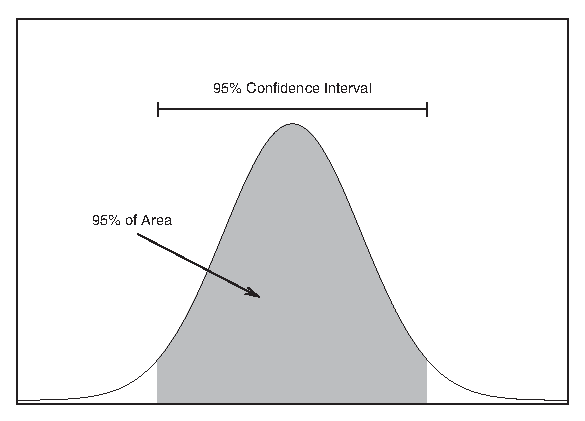
\includegraphics{img/confinterval}}
  \caption{The shaded area contains 95 percent of the area under the curve;
    the boundaries of the shaded region are the bounds on the 95 percent
    confidence interval.}
  \label{fig:confinterval}
\end{figure}
    
A similar concept can be applied to hypothesis testing, where sampling
distributions are often used to calculate so-called \emph{$p$-values}. \index{p-values@$p$-values} 
A $p$-value is an attempt to express the strength of the evidence in a\vadjust{\pagebreak}
hypothesis test and, in so doing, to soften the sharp binary
distinction between significant and not significant outcomes mentioned
earlier.  A $p$-value is \emph{the probability of obtaining a value as
  (or more) extreme than the one actually observed} under the
assumption that the null hypothesis is true (see Figure
\ref{fig:hypothesistest}). In other words, if the null hypothesis is
that there is no effect, and if the observed effect size is $x$, then
the $p$-value is the probability of observing an effect at least as
large as $x$. Obviously, a large effect is improbable (small
$p$-value) if the null hypothesis (zero effect) is true; hence a small
$p$-value is considered strong evidence against the null hypothesis.
However, a $p$-value is not ``the probability that the null hypothesis
is true''---such an interpretation (although appealing!) is incorrect.
The $p$-value is the probability of obtaining an effect as large or
larger than the observed one \emph{if} the null hypothesis is true.
(Classical statistics does not make probability statements about the
truth of hypotheses. Doing so would put us into the realm of Bayesian
statistics, a topic we will discuss toward the end of this chapter.)

\begin{figure}
  \centerline{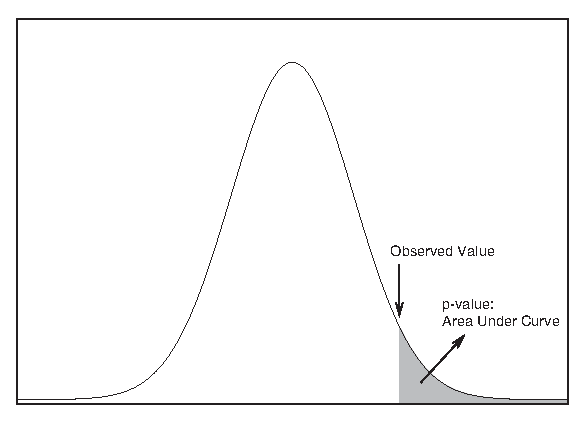
\includegraphics{img/testinterval}}
  \caption{The $p$-value is the probability of observing a value as
    large or larger than the one actually observed if the null
    hypothesis is true.}\label{fig:hypothesistest}\vspace*{-9pt}
\end{figure}

By the way, 
if you are thinking that this approach to hypothesis testing---with
its sliding $p$-values---is \index{sliding $p$-values} quite different from the cut-and-dried
significant--not significant approach discussed earlier, then you are
right. Historically, two competing theories of significance tests have
been developed and have generated quite a bit of controversy; even
today they sit a little awkwardly next to each other. (The approach
based on sliding $p$-values that need to be interpreted by the
researcher is due to Fisher; the decision-rule approach was developed
by Pearson and Neyman.) But enough, already. You can consult any
statistics book if you want to know more details.\vfill\pagebreak

\subsection{Example: Formal Tests Versus Graphical Methods}

\index{tests!versus graphical methods}
\index{graphical analysis!versus statistical tests}
  
Historically, classical statistics evolved as it did because working
with actual \emph{data} was hard. The early statisticians therefore
made a number of simplifying assumptions (mostly that data would be
normally distributed) and then proceeded to develop mathematical tools
(such as the sampling distributions introduced earlier in the chapter)
that allowed them to reason about data sets in a general way and
required only the knowledge of a few, easily calculated summary
statistics (such as the mean). The ingenuity of it all is amazing, but
it has led to an emphasis on formal technicalities as opposed to the
direct insight into the data. Today our situation is different, and we
should take full advantage of that.

An example will demonstrate what I mean. The listing below shows two
data sets. Are they the same, or are they different (in the sense that
their means are the same or different)?\footnote{This is a famous data
  set with history that is colorful but not really relevant here. A
  Web search for ``Quintus Curtius Snodgrass'' will turn up plenty of
  references.}
%
\begin{verbatim}
0.209         0.225
0.205         0.262
0.196         0.217	
0.210         0.240
0.202         0.230
0.207         0.229
0.224         0.235
0.223         0.217
0.220
0.201
\end{verbatim}
%
In case study 9.2.1 of their book, Larsen and Marx (see the
recommended reading at the end of this chapter) labor for several
pages and finally conclude that the data sets are different at the 99
percent level of significance.

Figure \ref{fig:snodgrass} shows a box plot for each of the data sets.
Case closed. \index{box-and-whisker plots!Quintus Curtius Snodgrass data sets} 

\begin{figure}
  \centerline{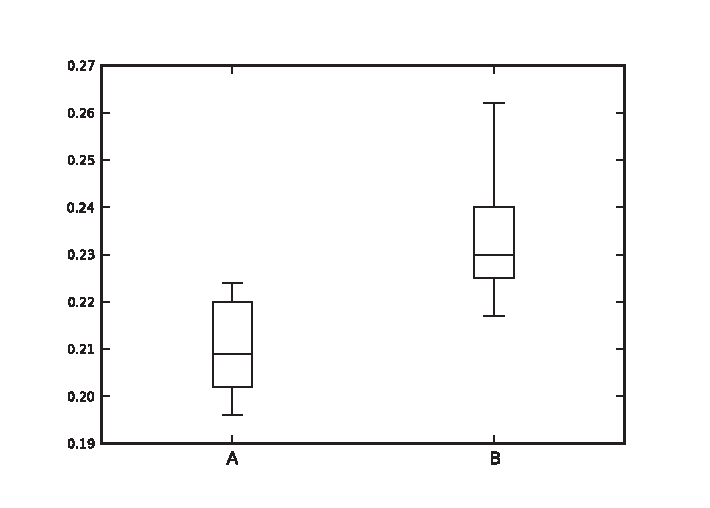
\includegraphics{img/snodgrass}}
  \caption{Box-and-whisker plots of the two Quintus Curtius Snodgrass
    data sets. There is almost no overlap between the two.}
  \label{fig:snodgrass}
\end{figure}

(In fairness, the formal test does something that a graphical method
cannot do: it gives us a quantitative criterion by which to make a
decision. I hope that the discussion in this chapter has convinced you
that this is not always an advantage, because it can lead to blind
faith in ``the number.'' Graphical methods require you to interpret
the results and take responsibility for the conclusions. Which is why
I like them: they keep you honest!)

\index{statistics!distributions|)}
\index{distributions!statistics|)}  

% ============================================================
\section{Controlled Experiments Versus Observational Studies}

\index{statistics!controlled experiments versus observational studies|(}
\index{experiments, versus observational studies|(}
 
Besides the machinery of formal statistical inference (using the
sampling distributions just discussed), the early statistics pioneers
also developed a general theory of how best to undertake statistical
studies. This conceptual framework is sometimes known as \emph{Design
  of Experiment} and is worth knowing about---not least because so
much of typical data mining activity does \emph{not} make use of it.

The most important distinction formalized by the Design of Experiment
theory is the one between an \emph{observational study} and a\vadjust{\pagebreak}
\emph{controlled experiment}. As the name implies, a controlled
experiment allows us to control many aspects of the experimental setup
and procedure; in particular, we control which treatment is applied to
which experimental unit (we will define these terms shortly).  For
example, in an agricultural experiment, we would treat some (but not
all) of the plots with a new fertilizer and then later compare the
yields from the two treatment groups. In contrast, with an
observational study, we merely collect data as it becomes (or already
is) available. In particular, retrospective studies are always
observational (not controlled).

In a controlled experiment, we are able to control the ``input'' of an
experiment (namely, the application of a treatment) and therefore can
draw much more powerful conclusions from the output. In contrast to
observational studies, a properly conducted controlled experiment can
provide strong support for cause-and-effect relationships between two
observations and can be used to rule out hidden (or confounding)
causes.  Observational studies can merely \emph{suggest} the existence
of a relationship between two observations; however, they can neither
prove that one observation is caused by the other nor rule out that
additional (unobserved) factors have played a role.

The following (intentionally whimsical) example will serve to make the
point. Let's say we have data that suggests that cities with many
lawyers also have many espresso stands and that cities with few
lawyers have few espresso stands. In other words, there is strong
correlation between the two quantities. But what conclusions can we
draw about the causal relationship between the two? Are lawyers
particularly high consumers of expensive coffee? Or does caffeine make
people more litigious? In short, there is no way for us to determine
what is cause and what is effect in this example. In contrast, if the
fertilized yields in the controlled agricultural experiment are higher
than the yields from the untreated control plots, we have strong
reason to conclude that this effect is due to the fertilizer
treatment.

In addition to the desire to establish that the treatment indeed
causes the effect, we also want to rule out the possibility of
additional, unobserved factors that might account for the observed
effect. Such factors, which influence the outcome of a study but are
not themselves part of it, are known as \emph{confounding} (or
``hidden'' or ``lurking'') variables.\index{confounding variables}\index{hidden variables}\index{lurking variables} In our agricultural example,
differences in soil quality might have a significant influence on the
yield---perhaps a greater influence than the fertilizer. The spurious
correlation between the number of lawyers and espresso stands is
almost certainly due to confounding: larger cities have more of
everything!  (Even if we account for this effect and consider the per
capita \emph{density} of lawyers and espresso stands, there is still a
plausible confounding factor: the income generated per head in the
city.) In the next section, we will discuss how \emph{randomization}
can help to remove the effect of confounding variables.

The distinction between controlled experiments and observational
studies is most critical. Many of the most controversial scientific or
statistical issues involve observational studies. In particular,
reports in the mass media often concern studies that (inappropriately)
draw causal inferences from observational\vadjust{\pagebreak} studies (about topics such
as the relationship between gun laws and homicide rates, for example).
Sometimes controlled experiments are not possible, with the result
that it becomes almost impossible to settle certain questions once and
for all. (The controversy around the connection between smoking and
lung cancer is a good example.)

In any case, make sure you understand clearly the difference between
controlled and observational studies, as well as the fundamental
limitations of the latter!

\vspace*{-9pt}
\subsection{Design of Experiments}

In a controlled experiment, we divide the \emph{experimental units}
that constitute our sample into two or more groups and then apply
different \emph{treatments} or \emph{treatment levels} to the units in
each group. In our agricultural example, the plots correspond to the
experimental units, fertilization is the treatment, and the options
``fertilizer'' and ``no fertilizer'' are the treatment levels.

\enlargethispage{6pt}

Experimental design involves several techniques to improve the quality
and reliability of any conclusions drawn from a controlled experiment.

\begin{unnumlist}
\subparagraph{Randomization}\vspace*{2pt} 
Randomization \index{randomization} means that treatments (or treatment
  levels) are assigned to experimental units in a random fashion.
  Proper randomization suppresses systematic errors. (If we assign
  fertilizer treatment randomly to plots, then we remove the
  systematic influence of soil quality, which might otherwise be a
  confounding factor, because high-quality and low-quality plots are
  now equally likely to receive the fertilizer treatment.) Achieving
  true randomization is not as easy as it looks---I'll come back to
  this point shortly.

\subparagraph{Replication}\vspace*{2pt} 
Replication \index{replication} means that the same treatment is
  applied to more than one experimental unit. Replication serves to
  reduce the variability of the results by averaging over a larger
  sample.  Replicates should be independent of each other, since
  nothing is gained by repeating the same experiment on the same unit
  multiple times.

\subparagraph{Blocking}\vspace*{2pt}
We \index{blocking} sometimes know (or at least strongly suspect) that
  not all experimental units are equal. In this case, it may make
  sense to group equivalent experimental units into ``blocks'' and
  then to treat each such block as a separate sample. For example, if
  we know that plots A and C have poor soil quality and that B and D
  have better soil, then we would form two blocks---consisting of
  (A, C) and (B, D), respectively---before proceeding to make a
  randomized assignment of treatments \emph{for each block
    separately}.  Similarly, if we know that web traffic is
  drastically different in the morning and the afternoon, we should
  collect and analyze data for both time periods separately. This also
  is a form of blocking.

\subparagraph{Factorization}\vspace*{2pt}
The \index{factorization} last of these techniques applies only to
  experiments involving several treatments (\eg, irrigation and
  fertilization, to stay\vadjust{\pagebreak} within our agricultural framework). The
  simplest experimental design would make only a single change at any
  given time, so that we would observe yields with and without
  irrigation as well as with and without fertilizer. But this approach
  misses the possibility that there are \emph{interactions} between
  the two treatments---for example, the effect of the fertilizer may
  be significantly higher when coupled with improved irrigation.
  Therefore, in a factorial experiment all possible combinations of
  treatment levels are tried. Even if a fully factorial experiment is
  not possible (the number of combinations goes up quickly as the
  number of different treatments grows), there are rules for how best
  to select combinations of treatment levels for drawing optimal
  conclusions from the study.
\end{unnumlist}

Another term you may come across in this context is ANOVA (analysis of
variance), \index{ANOVA (analysis of variance)} which is a standard way of summarizing results from
controlled experiments. It emphasizes the variations within each
treatment group for easy comparison with the variances between the
treatments, so that we can determine whether the differences between
different treatments are significant compared to the variation within
each treatment group. ANOVA is a clever bookkeeping technique, but it
does not introduce particularly noteworthy new statistical concepts.

A word of warning: when conducting a controlled experiment, make sure
that you apply the techniques properly; in particular, beware of
\emph{pseudo-randomization} and \emph{pseudo-replication}. \index{pseudo-randomization} \index{pseudo-replication}  

Pseudo-randomization occurs if the assignment of treatments to
experimental units is not truly random. This can occur relatively
easily, even if the assignment \emph{seems} to be random.  For
example, if you would like to try out two different drugs on lab rats,
it is not sufficient to ``pick a rat at random'' from the cage to
administer the treatment. What does ``at random'' mean? It might very
well mean picking the most active rat first because it comes to the
cage door. Or maybe the least aggressive-looking one. In either case,
there is a systematic bias!

Here is another example, perhaps closer to home: the web-lab. Two
different site designs are to be presented to viewers, and the
objective is to measure conversion rate or click-throughs or some
other metric.  There are multiple servers, so we dedicate one of them
(chosen ``at random'') to serve the pages with the new design. What's
wrong with that?

\emph{Everything!} Do you have any indication that web requests are
assigned to servers in a random fashion? Or might servers have, for
example, a strong geographic bias? Let's assume the servers are
behind some ``big-IP'' box that routes requests to the servers. How is
the routing conducted---randomly, or round-robin, or based on traffic
intensity? Is the routing smart, so that servers with slower response
times get fewer hits? What about sticky sessions, and what about the
relationship between sticky sessions and slower response times? Is the
router reordering the incoming requests in some way?  That's a lot of
questions---questions that randomization is intended to \emph{avoid}.
In fact, you are not running a controlled experiment at all: you are
conducting an observational study!

The only way that I know to run a controlled experiment is by deciding
ahead of time which experimental unit will receive which treatment. In
the lab rat example, rats should have been labeled and then treatments
assigned to the labels using a (reliable) random number generator or
random table. In the web-server example it is harder to achieve true
randomization, because the experimental units are not known ahead of
time. A simple rule (\eg, show the new design to every $n$th request)
won't work, because there may be significant correlation between
subsequent requests. It's not so easy.

Pseudo-replication occurs when experimental units are not truly
independent. Injecting the same rat five times with the same drug does
not reduce variability! Similarly, running the same query against a
database could be misleading because of changing cache utilization.
And so on. In my experience, pseudo-replication is easier to spot and
hence tends to be less of a problem than pseudo-randomization.

Finally, I should mention one other term that often comes up in the
context of proper experimental process: \emph{blind} \index{blind experiments} and
\emph{double-blind} experiments. \index{double-blind experiments} In a blind experiment, the
experimental unit should not know which treatment it receives; in a
double-blind experiment, the investigator---at the time of the
experiment---does not know either.  The purpose of blind and
double-blind experiments is to prevent the knowledge of the treatment
level from becoming a confounding factor. If people know that they
have been given a new drug, then this knowledge itself may contribute
to their well-being. An investigator who  knows which field is receiving
the fertilizer might weed that particular field more vigorously and
thereby introduce some invisible and unwanted bias. Blind experiments
play a huge role in the medical field but can also be important in
other contexts.  However, I would like to emphasize that the question
of ``blindness'' (which concerns the experimental procedure) is a
different issue than the Design of Experiment prescriptions (which are
intended to reduce statistical uncertainty).
    
\vspace*{-9pt}
\subsection{Perspective}

It is important to maintain an appropriate perspective on these
matters.

In practice, many studies are observational, not controlled.
Occasionally, this is a painful loss and only due to the inability to
conduct a proper controlled experiment (smoking and lung cancer,
again!). Nevertheless, observational studies can be of great value:
one reason is that they may be exploratory and discover new and
previously unknown behavior. In contrast, controlled experiments are
always confirmatory in deciding between the effectiveness or
ineffectiveness of a specific ``treatment.''

Observational studies can be used to derive predictive models even
while setting aside the question of causation. The machine-learning
community, for instance, attempts to develop \emph{classification}
algorithms that use descriptive attributes or \emph{features} of the
unit to predict whether the unit belongs to a given class. They work
entirely without controlled experiments and have developed methods for
quantifying the accuracy of their results. (We will describe some in
Chapter \ref{ch:prediction}.)

That being said, it is important to understand the limitations of
observational studies---in particular, their inability to support
strong conclusions regarding cause-and-effect relationships and their
inability to rule out confounding factors. In the end, the power of
controlled experiments can be their limitation, because such
experiments require a level of control that limits their application.
% to areas that aren't that contentious to begin with.

\index{statistics!controlled experiments versus observational studies|)}
\index{experiments, versus observational studies|)}

% ============================================================
\section{Optional: Bayesian Statistics�The Other Point of View}

\index{statistics!Bayesian statistics|(} 
\index{Bayesian statistics|(} 

There is an alternative approach to statistics that is based on a
different interpretation of the concept of \emph{probability} itself.
This may come as a surprise, since probability seems to be such a
basic concept.  The problem is that, although we have a very strong
intuitive sense of what we mean by the word ``probability,'' it is not
so easy to give it a rigorous meaning that can be used to develop a
mathematical theory.

The interpretation of probability used by classical statistics (and,
to some degree, by abstract probability theory) treats probability as
a \emph{limiting frequency}: if you toss a fair coin ``a large number
of times,'' then you will obtain Heads about half of the time; hence
the probability for Heads is $1/2$. Arguments and theories starting
from this interpretation are often referred to as ``frequentist.''

An alternative interpretation of probability views it as the
degree of our ignorance about an outcome: since we don't know which
side will be on top in the next toss of a fair coin, we assign
each possible outcome the same probability---namely $1/2$. We can
therefore make statements about the probabilities associated with
individual events without having to invoke the notion of a large
number of repeated trials. Because this approach to probability and
statistics makes use of \emph{Bayes' theorem} at a central step in
its reasoning, it is usually called \emph{Bayesian statistics} and
has become increasingly popular in recent years. Let's compare the
two interpretations in a bit more detail.

\subsection{The Frequentist Interpretation of Probability}

\index{Bayesian statistics!frequentist interpretation of probability} 
\index{frequentist interpretation of probability}
\index{probability!frequentist interpretation}  

In the frequentist interpretation, probability is viewed as the
limiting frequency of each outcome of an experiment that is repeated a
large number of times.  This ``frequentist'' interpretation is the
reason for some of the peculiarities of classical statistics. For
example, in classical statistics it is incorrect to say that a 95
percent confidence interval for some parameter has a 95 percent chance
of containing the true value---after all, the true value is either
contained in the interval or not; period. The only statement that we
can make is that, if we perform an experiment to measure this
parameter many times, then in about 95 percent of all cases the
experiment will yield a value for this parameter that lies within the
95 percent confidence interval.

This type of reasoning has a number of drawbacks.

\begin{itemize}
\item It is awkward and clumsy, and liable to (possibly even
  unconscious) misinterpretations.

\item The constant appeal to a ``large number of trials'' is
  artificial even in situations where such a sequence of trials
  would---at least in principle---be possible (such as tossing a coin).
  But it becomes wholly ficticious in situations where the trial
  cannot possibly be repeated. The weather report may state: ``There
  is an 80 percent chance of rain tomorrow.'' What is that supposed to
  mean? It is either going to rain tomorrow or not!  Hence we must
  again invoke the unlimited sequence of trials and say that in 8 out
  of 10 cases where we observe the current meteorological conditions,
  we expect rain on the following day. But even this argument is
  illusionary, because we will never observe these \emph{precise}
  conditions ever again: that's what we have been learning from chaos
  theory and related fields.

\item We would frequently like to make statements such as the one
  about the chance of rain, or similar ones---for example, ``The
  patient has a 60 percent survival probability,'' and ``I am 25
  percent certain that the contract will be approved.''  In all such
  cases the actual outcome is not of a probabilistic nature: it will
  rain or it will not; the patient will survive or not; the contract
  will be approved or not. Even so, we'd like to express a degree of
  certainty about the expected outcome even if appealing to an
  unlimited sequence of trials is neither practical nor even
  meaningful.
\end{itemize}

From a strictly frequentist point of view, a statement like ``There is
an 80 percent chance of rain tomorrow'' is nonsensical. Nevertheless,
it seems to make so much intuitive sense. In what way can this
intuition be made more rigorous? This question leads us to
\emph{Bayesian statistics} or \emph{Bayesian reasoning}.

\subsection{The Bayesian Interpretation of Probability}

\index{Bayesian statistics!Bayesian interpretation of probability}
\index{probability!Bayesian interpretation}
  
To understand the Bayesian point of view, we first need to review the
concept of \emph{conditional probability}. \index{conditional probability} The conditional probability
$P(A|B)$ gives us the probability for the event $A$, \emph{given} (or
assuming) that event $B$ has occurred. You can easily convince
yourself that the following is true:
%
\[
P( A | B ) = \frac{ P( A \cap B ) }{ P( B ) }
\]
%
where $P( A \cap B )$ is the \emph{joint probability} \index{joint probability} of finding both
event $A$ and event $B$. For example, it is well known that men are
much more likely than women to be color-blind: about 10 percent of men
are color-blind but fewer than 1 percent of women are color-blind.
These are \emph{conditional} probabilities---that is, the probability
of being color-blind \emph{given} the gender:
\begin{gather*}
P( \text{color-blind} | \text{male} ) = 0.1 \\
P( \text{color-blind} | \text{female} ) = 0.01 
\end{gather*}

In contrast, if we ``randomly'' pick a person off the street, then we
are dealing with the \emph{joint} probability that this person is
color-blind \emph{and} male.\vadjust{\pagebreak} The person has a 50 percent chance of
being male and a 10 percent conditional probability of being
color-blind, given that the person is male. Hence, the joint
probability for a random person to be color-blind \emph{and} male is 5
percent, in agreement with the definition of conditional probability
given previously.

One can now rigorously prove the following equality, which is known as
\emph{Bayes' theorem}:
%
\[
P( A | B ) = \frac{ P( B | A ) P( A ) }{ P( B ) }
\]
%
In words: the probability of finding $A$ given $B$ is equal to the
probability of finding $B$ given $A$ multiplied by the probability of
finding $A$ and divided by the probability of finding $B$.

Now, let's return to statistics and data analysis. Assume there is
some parameter that we attempt to determine through an experiment
(say, the mass of the proton or the survival rate after surgery).  We
are now dealing with two ``events'': event $B$ is the occurrence of
the specific set of measurements that we have observed, and the
parameter taking some specific value constitutes event $A$.  We can
now rewrite Bayes' theorem as follows:
%
\[
P( \text{\textit{parameter}} | \text{\textit{data}} )
\propto
P( \text{\textit{data}} | \text{\textit{parameter}} ) 
P( \text{\textit{parameter}} )
\]
%
(I have dropped the denominator, which I can do because the
denominator is simply a constant that does not depend on the parameter
we wish to determine. The left- and righthand sides are now no longer
equal, so I have replaced the equality sign with $\propto$ to indicate
that the two sides of the expression are merely proportional: equal to
within a numerical constant.)

Let's look at this equation term by term. 

On the lefthand side, we have \emph{the probability of finding a
  certain value for the parameter, given the data}. That's pretty
exciting, because this is an expression that makes an explicit
statement about the \emph{probability} of an event (in this case, that
the parameter has a certain value), given the data. This probability
is called the \emph{posterior probability}, \index{posterior probability (posterior probability distribution)} or simply \emph{the
  posterior}, and is defined solely through Bayes' theorem without
reference to any unlimited sequence of trials.  Instead, it is a
measure of our ``belief'' or ``certainty'' about the outcome (\ie, the
value of the parameter) given the data.

The first term on the righthand side, $P( \text{\textit{data}} |
\text{\textit{parameter}} )$, is known as the \emph{likelihood
  function}. \index{likelihood function} This is a mathematical expression that links the
parameter to the probability of obtaining specific data points in an
actual experiment.  The likelihood function constitutes our ``model''
for the system under consideration: it tells us what data we can
expect to observe, given a particular value of the parameter. (The
example in the next section will help to clarify the meaning of this
term.)

Finally, the term $P( \text{\textit{parameter}} )$ is known as the
\emph{prior probability}, \index{prior probability} or simply \emph{the prior}, and~captures our
``prior'' (prior to the experiment) belief of finding a certain
outcome---specifically our prior\vadjust{\pagebreak} belief that the parameter has a
certain value.  It is the existence of this prior that makes the
Bayesian approach so controversial, because it seems to introduce an
inappropriately subjective element into the analysis. In reality,
however, the influence of the prior on the final result of the
analysis is typically small, in particular when there is plenty of
data. One can also find so-called ``noninformative'' priors that
express our complete ignorance about the possible outcomes. But the
prior is there, and it forces us to think about our assumptions
regarding the experiment and to state some of these assumptions
explicitly (in form of the prior distribution function).

\subsection{Bayesian Data Analysis: A Worked Example}

\index{Bayesian statistics!data analysis example|(}
 
All of this will become much clearer once we demonstrate these
concepts in an actual example. The example is very simple, so as not
to distract from the concepts.

Assume we have a coin that has been tossed 10 times, producing the
following set of outcomes (H for Heads, T for Tails):\vspace*{9pt}

\begin{verbatim}
T H H H H T T H H H
\end{verbatim}

If you count the outcomes, you will find that we obtained 7 Heads and
3 Tails in 10 tosses of the coin.

Given this data, we would like to determine whether the coin is fair
or not. Specifically, we would like to determine the probability $p$
that a toss of this coin will turn out Heads. (This is the
``parameter'' we would like to estimate.) If the coin is fair, then
$p$ should be close to $1/2$.

Let's write down Bayes' equation, adapted to this system:
%
\[
P( p | \braces{\text{T H H H H T T H H H}} ) 
  \propto P( \braces{\text{T H H H H T T H H H}} | p ) P( p )
\]
%
Notice that at this point, the problem has become \emph{parametric}.
All that is left to do is to determine the value of the parameter $p$
or, more precisely, the posterior probability distribution for all
values of $p$.

To make progress, we need to supply the likelihood function and the
prior. Given this system, the likelihood function is particularly
simple: $P(\text{H} | p ) = p$ and $P(\text{T} | p ) = 1-p$.  You
should convince yourself that this choice of likelihood function gives
us exactly what we want: the probability to obtain Heads or Tails,
given $p$.

We also assume that the tosses are independent, which implies that
only the total number~of Heads or Tails matters but not the order in
which they occurred.  Hence we don't need to find the combined
likelihood for the specific sequence of 10 tosses; instead, the
likelihood of the set of events is simply the product of the 10
individual tosses. (The likelihood ``factors'' for independent
events---this argument occurs frequently in Bayesian analysis.)

Finally, we know nothing about this coin. In particular, we have no
reason to believe that any value of $p$ is more likely than any other,
so we choose as prior probability distribution the ``flat'' distribution
$P(p) = 1$ for all $p$.

Collecting everything, we end up with the following expression (where
I have dropped some combinatorial factors that do not depend on $p$):
%
\[
P( p | \braces{ \text{7 Heads, 3 Tails} } ) \propto p^7 (1-p)^3
\]
%
This is the posterior probability distribution\index{posterior probability (posterior probability
distribution)}\index{distributions!posterior probability distribution} for the parameter $p$
based on the experimental data (see Figure \ref{fig:bayes1}). We can see that it has a peak near
$p=0.7$, which is the most probable value for $p$.  Note that the absence of tick marks on the $y$
axis in Figure \ref{fig:bayes1}: the denominator, which we dropped earlier, is
still undetermined, and therefore the overall scale of the function is
not yet fixed. If we are interested only in the \emph{location} of the
maximum, this does not matter.

\begin{figure}
  \centerline{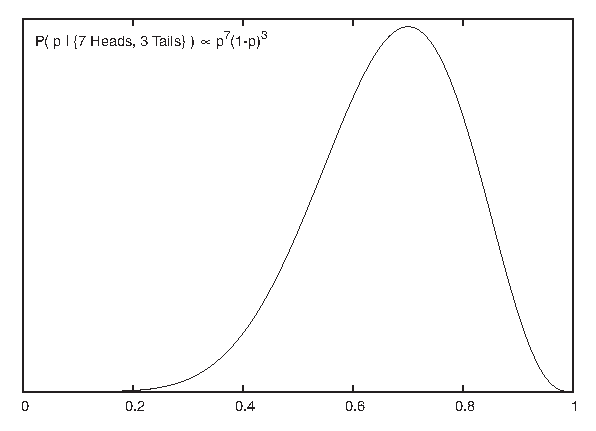
\includegraphics{img/bayes1}}
  \caption{The (unnormalized) posterior probability of obtaining 7
    Heads in 10 tosses of a coin as a function of $p$.}
  \label{fig:bayes1}
\end{figure}

But we are not restricted to a single (point) estimate for $p$---the
entire distribution function is available to us! We can now use it to
construct confidence intervals for $p$. And because we are now talking
about Bayesian probabilities, it would be legitimate to state that
``the confidence interval has a 95 percent chance of containing the
true value of $p$.''

We can also evaluate any function that depends on $p$ by integrating
it against the posterior distribution for\vadjust{\pagebreak} $p$. As a particularly
simple example, we could calculate the expectation value of $p$ to
obtain the single ``best'' estimate of $p$ (rather than use the most
probable value as we did before):
%
\[
E[p] 
= \frac{\int \! p \, P(p | \braces{ \text{7 Heads, 3 Tails} }) \rms{p} }
       {\int \! P(p | \braces{ \text{7 Heads, 3 Tails} }) \rms{p} }
\]
%
Here we finally need to worry about all the factors that we dropped
along the way, and the denominator in the formula is our way of fixing
the normalization ``after the fact.'' To ensure that the probability
distribution is properly normalized, we divide explicitly by the
integral over the whole range of values, thereby guaranteeing that the
total probability equals $1$ (as it must).

It is interesting to look at the roles played by the likelihood and
the prior in the result. In Bayesian analysis, the posterior
``interpolates'' between the prior and the data-based likelihood
function. If there is only very little data, then the likelihood
function will be relatively flat, and therefore the posterior will be
more influenced by the prior. But as we collect more data (\ie, as the
empirical evidence becomes stronger), the likelihood function becomes
more and more narrowly peaked at the most likely value of $p$,
regardless of the choice of prior. Figure \ref{fig:bayes2}
demonstrates this effect. It shows the posterior for a total of 10
trials and a total of 30 trials (while keeping the same ratio of Heads
to Tails): as we gather more data, the uncertainty in the resulting
posterior shrinks.

\begin{figure}
  \centerline{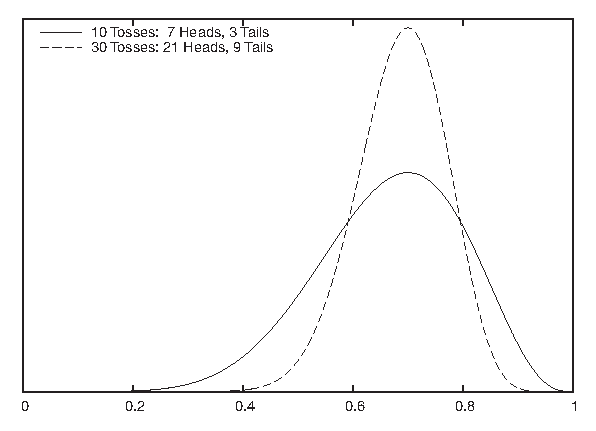
\includegraphics{img/bayes2}}
  \caption{The (unnormalized) posterior probability of obtaining 70
    percent Heads in 10 and in 30 tosses of a coin. The more data
    there is, the more strongly peaked the posterior distribution
    becomes.}
  \label{fig:bayes2}
\end{figure}\pagebreak

Finally, Figure \ref{fig:bayes3} demonstrates the effect of the prior.
Whereas the posterior distributions shown in Figure \ref{fig:bayes2}
were calculated using a flat prior, those in Figure \ref{fig:bayes3}
were calculated using a Gaussian prior---which expresses a rather
strong belief that the value of $p$ will be between $0.35$ and $0.65$.
The influence of this prior belief is rather significant for the
smaller data set, but as we take more and more data points, its
influence is increasingly diminished.

\begin{figure}
  \centerline{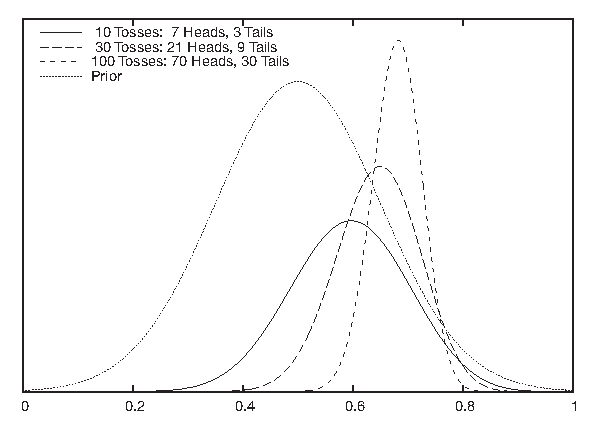
\includegraphics{img/bayes3}}
  \caption{The effect of a nonflat prior: posterior probabilities for
    data sets of different sizes, calculated using a Gaussian prior.}
  \label{fig:bayes3}
\end{figure}

\index{Bayesian statistics!data analysis example|)}

\subsection{Bayesian Inference: Summary and Discussion}

\index{Bayesian statistics!inference}
 
Let's summarize what we have learned about Bayesian data analysis or
\emph{Bayesian inference} and discuss what it can do for us---and what
it can't.

First of all, the Bayesian (as opposed to the frequentist) approach to
inference allows us to compute a true probability distribution for any
parameter in question. This has great intuitive appeal, because it
allows us to make statements such as ``There is a 90 percent chance of
rain tomorrow'' without having to appeal to the notion of extended
trials of identical experiments.

The posterior probability distribution\index{posterior probability (posterior probability
distribution)}\index{distributions!posterior probability distribution} arises as the product of
the likelihood function \index{likelihood function} and the prior. The likelihood links
experimental results to values of the parameter, and the prior expresses our previous knowledge or
belief about the parameter.

The Bayesian approach has a number of appealing features. Of course,
there is the intuitive nature of the results\vadjust{\pagebreak} obtained using Bayesian
arguments: real probabilities and 95 percent confidence intervals
that have exactly the kind of interpretation one would expect!
Moreover, we obtain the posterior probability distribution in full
generality and without having to make limiting assumptions (\eg,
having to assume that the data is normally distributed).

Additionally, the likelihood function enters the calculation in a way
that allows for great flexibility in how we build ``models.'' Under
the Bayesian approach, it is very easy to deal with missing data, with
data that is becoming available over time, or with heterogeneous data
sets (\ie, data sets in which different attributes are known about
each data point). Because the result of Bayesian inference is a
probability distribution itself, it can be used as input for a new
model that builds on the previous one (hierarchical models). Moreover,
we can use the prior to incorporate previous (domain) knowledge that
we may have about the problem under consideration.

On the other hand, Bayesian inference has some problems, too---even
when we concentrate on practical applications only, leaving the entire
philosophical debate about priors and subjectivity aside.

First of all, Bayesian inference is always \emph{parametric}; it is
never just exploratory or descriptive. Because Bayesian methods force
us to supply a likelihood function explicitly, they force us to be
specific about our choice of model assumptions: we must already have a
likelihood function in mind, for otherwise we can't even get started
(hence such analysis can never be exploratory).  Furthermore, the
result of a Bayesian analysis is always a posterior
distribution---that is, a conditional probability of \emph{something},
given the data. Here, that ``something'' is some form of hypothesis
that we have, and the posterior gives us the probability that this
hypothesis is true. To make this prescription operational (and, in
particular, expressible through a likelihood function), we pretty much
have to parameterize the hypothesis. The inference then consists of
finding the best value for this parameter, given the data---which is a
parametric problem, given a specific choice for the model (\ie, the
likelihood function). (There are so-called ``nonparametric'' Bayesian
methods, but in reality they boil down to parametric models with very
large numbers of parameters.)

Additionally, actual Bayesian calculations are often difficult.
Recall that Bayesian inference gives us the full explicit posterior
distribution function.  If we want to summarize this function, we
either need to find its maximum or integrate it to obtain an
expectation value.  Both of these problems are hard, especially when
the likelihood function is complicated and there is more than one
parameter that we try to estimate. Instead of explicitly integrating
the posterior, one can \emph{sample} it---that is, draw random points
that are distributed according to the posterior distribution, in order
to evaluate expectation values.  This is clearly an expensive process
that requires computer time and specialized software (and the
associated know-how).  There can also be additional problems. For
example, if the parameter space is very high-dimensional, then
evaluating the likelihood function (and hence the posterior) may be
difficult.

In contrast, frequentist methods tend to make more assumptions up
front and rely more strongly on general analytic results and
approximations. With frequentist methods, the hard work has typically
already been done (analytically), leading to an asymptotic or
approximate formula that you only need to plug in. Bayesian methods
give you the full, nonapproximate result but leave it up to you to
evaluate it.  The disadvantage of the plug-in approach, of course, is
that you might be plugging into an inappropriate formula---because
some of the assumptions or approximations that were used to derive it
do not apply to your system or data set.

To bring this discussion to a close, I'd like to end with a cautionary
note. Bayesian methods are very appealing and even
exciting---something that is rarely said about classical frequentist
statistics.  On the other hand, they are probably not very suitable
for casual uses.

\begin{itemize}
\item Bayesian methods are parametric and specific; they are never
  exploratory or descriptive. If we already know what specific
  question to ask, then Bayesian methods may be the best way of
  obtaining an answer. But if we don't yet know the proper questions
  to ask, then Bayesian methods are not applicable.

\item Bayesian methods are difficult and require a fair deal of
  sophistication, both in setting up the actual model (likelihood
  function and prior) and in performing the required calculations.
\end{itemize}

As far as results are concerned, there is not much difference between
frequentist and Bayesian analysis. When there is sufficient data (so
that the influence of the prior is small), then the end results are
typically very similar, whether they were obtained using frequentist
methods or Bayesian methods.

Finally, you may encounter some other terms and concepts in the
literature that also bear the ``Bayesian'' moniker: Bayesian
classifier, Bayesian network, Bayesian risk, and more.  Often, these
have nothing to do with Bayesian (as opposed to frequentist) inference
as explained in this chapter.  Typically, these methods involve
conditional probabilities and therefore appeal at some point to Bayes'
theorem.  A Bayesian classifier, for instance, is the conditional
probability that an object belongs to a certain class, given what we
know about it. A Bayesian network is a particular way of organizing
the causal relationships that exist among events that depend on many
interrelated conditions. And so on.

\index{Bayesian statistics|)} 
\index{statistics!Bayesian statistics|)} 

% ============================================================
\section{Workshop: R}

\index{statistics!R statistical analysis package|(} 
\index{R statistical analysis package|(}
\index{software!R statistical analysis package|(} 
 
R is an environment for data manipulation and numerical calculations,
specifically statistical applications. Although it can be used in a
more general fashion for programming or computation, its real strength
is the large number of built-in (or user-contributed) statistical
functions.

R is an open source clone of the S programming language, which was
originally developed at Bell Labs in the 1970s. It was one of the
first environments to combine the capabilities that today we expect
from a scripting language (\eg, memory management, proper strings,
dynamic typing, easy file handling) with integrated graphics and 
intended for an interactive usage pattern. 

I tend to stress the word \emph{environment} when referring to R,
because the way it integrates its various components is essential to
R. It is misleading to think of R as a programming language that also
has an interactive shell (like Python or Groovy). Instead, you might
consider it as a shell but for handling data instead of files.
Alternatively, you might want to view R as a text-based spreadsheet on
steroids. The ``shell'' metaphor in particular is helpful in
motivating some of the design choices made by R.

The essential data structure offered by R is the so-called \emph{data
  frame}. \index{data frames} A data frame encapsulates a data set and is the central
abstraction that R is built on. Practically all operations involve the
handling and manipulation of frames in one way or the other.

Possibly the best way to think of a data frame is as being comparable
to a \emph{relational database table}. Each data frame is a
rectangular data structure consisting of rows and columns.  Each
\emph{column} has a designated data type, and all entries in that
column must be of that type. Consequently, each \emph{row} will in
general contain entries of different types (as defined by the types of
the columns), but all rows must be of the same form. All this should
be familiar from relational databases. The similarities continue:
operations on frames can either project out a subset of columns, or
filter out a subset of rows; either operation results in a new data
frame. There is even a command (\texttt{merge}) that can perform a
join of two data frames on a common column.  In addition (and in
contrast to databases), we will frequently \emph{add} columns to an
existing frame---for example, to hold the results of an intermediate
calculation.

We can refer to columns by name. The names are either read from the
first line of the input file, or (if not provided) R will substitute
synthetic names of the form \texttt{V1}, \texttt{V2}, \dots.  In
contrast, we filter out a set of rows through various forms of
``indexing magic.'' Let's look at some examples.

Consider the following input file:\vspace*{9pt}

\begin{verbatim}
Name    Height  Weight  Gender
Joe     6.2     192.2   0
Jane    5.5     155.4   1
Mary    5.7     164.3   1
Jill    5.6     166.4   1
Bill    5.8     185.8   0
Pete    6.1     201.7   0
Jack    6.0     195.2   0
\end{verbatim}

Let's investigate this data set using R, placing particular emphasis
on how to handle and manipulate data with R---the full session\vadjust{\pagebreak}
transcript is included below.  The commands entered at the command
prompt are prefixed by the prompt \texttt{>}, while R output is shown
without the prompt:

\begin{verbatim}
> d <- read.csv( "data", header = TRUE, sep = "\t" )
> str(d)
'data.frame':   7 obs. of  4 variables:
 $ Name  : Factor w/ 7 levels "Bill","Jack",..: 5 3 6 4 1 7 2
 $ Height: num  6.2 5.5 5.7 5.6 5.8 6.1 6
 $ Weight: num  192 155 164 166 186 ...
 $ Gender: int  0 1 1 1 0 0 0
> 
> mean( d$Weight )
[1] 180.1429
> mean( d[,3] )
[1] 180.1429
> 
> mean( d$Weight[ d$Gender == 1 ] )
[1] 162.0333
> mean( d$Weight[ 2:4 ] )
[1] 162.0333
> 
> d$Diff <- d$Height - mean( d$Height )
> print(d)
  Name Height Weight Gender        Diff
1  Joe    6.2  192.2      0  0.35714286
2 Jane    5.5  155.4      1 -0.34285714
3 Mary    5.7  164.3      1 -0.14285714
4 Jill    5.6  166.4      1 -0.24285714
5 Bill    5.8  185.8      0 -0.04285714
6 Pete    6.1  201.7      0  0.25714286
7 Jack    6.0  195.2      0  0.15714286
> summary(d)
   Name       Height          Weight          Gender            Diff         
 Bill:1   Min.   :5.500   Min.   :155.4   Min.   :0.0000   Min.   :-3.429e-01
 Jack:1   1st Qu.:5.650   1st Qu.:165.3   1st Qu.:0.0000   1st Qu.:-1.929e-01
 Jane:1   Median :5.800   Median :185.8   Median :0.0000   Median :-4.286e-02
 Jill:1   Mean   :5.843   Mean   :180.1   Mean   :0.4286   Mean   : 2.538e-16
 Joe :1   3rd Qu.:6.050   3rd Qu.:193.7   3rd Qu.:1.0000   3rd Qu.: 2.071e-01
 Mary:1   Max.   :6.200   Max.   :201.7   Max.   :1.0000   Max.   : 3.571e-01
 Pete:1                                                                      
> 
> d$Gender <- factor( d$Gender, labels = c("M", "F") )
> summary(d)
   Name       Height          Weight      Gender      Diff           
 Bill:1   Min.   :5.500   Min.   :155.4   M:4    Min.   :-3.429e-01  
 Jack:1   1st Qu.:5.650   1st Qu.:165.3   F:3    1st Qu.:-1.929e-01  
 Jane:1   Median :5.800   Median :185.8          Median :-4.286e-02  
 Jill:1   Mean   :5.843   Mean   :180.1          Mean   : 2.538e-16  
 Joe :1   3rd Qu.:6.050   3rd Qu.:193.7          3rd Qu.: 2.071e-01  
 Mary:1   Max.   :6.200   Max.   :201.7          Max.   : 3.571e-01  
 Pete:1                                                              
> 
> plot( d$Height ~ d$Gender )
> plot( d$Height ~ d$Weight, xlab="Weight", ylab="Height" )
\end{verbatim}
\begin{verbatim}
> m <- lm( d$Height ~ d$Weight )
> print(m)

Call:
lm(formula = d$Height ~ d$Weight)

Coefficients:
(Intercept)     d$Weight  
    3.39918      0.01357  

> abline(m)
> abline( mean(d$Height), 0, lty=2 )
\end{verbatim}\vspace*{-3pt}

Let's step through this session in some detail and explain what is 
going on.

First, we read the file in and assign it to the variable \texttt{d},
which is a data frame as discussed previously. The function
\texttt{str(d)} shows us a string representation of the data frame. We
can see that the frame consists of five named columns, and we can also
see some typical values for each column.  Notice that R has assigned a
data type to each column: height and weight have been recognized as
floating-point values; the names are considered a ``factor,'' which is
R's way of indicating a categorical variable; and finally the gender
flag is interpreted as an integer. This is not ideal---we will come
back to that.

\begin{verbatim}
> d <- read.csv( "data", header = TRUE, sep = "\t" )
> str(d)
'data.frame':   7 obs. of  4 variables:
 $ Name  : Factor w/ 7 levels "Bill","Jack",..: 5 3 6 4 1 7 2
 $ Height: num  6.2 5.5 5.7 5.6 5.8 6.1 6
 $ Weight: num  192 155 164 166 186 ...
 $ Gender: int  0 1 1 1 0 0 0
\end{verbatim}\vspace*{-3pt}

Let's calculate the mean of the weight column to demonstrate some
typical ways in which we can select rows and columns. The most
convenient way to specify a column is by name: \texttt{d\$Weight}. The
use of the dollar-sign (\texttt{\$}) to access members of a data
structure is one of R's quirks that one learns to live with. Think of
a column as a shell variable!  (By contrast, the dot (\texttt{.}) is
not an operator and can be part of a variable or function name---in
the same way that an underscore (\texttt{\_}) is used in other
languages. Here again the shell metaphor is useful: recall that shells
allow the dot as part of filenames!)

\begin{verbatim}
> mean( d$Weight )
[1] 180.1429
> mean( d[,3] )
[1] 180.1429
\end{verbatim}\vspace*{-3pt}

Although its name is often the most convenient method to specify a
column, we can also use its numeric index. Each element in a data
frame can be accessed using its row and column index via the familiar
bracket notation: \texttt{d[row,col]}. Keep in mind that the vertical
(row) index comes first, followed by the horizontal (column) index.
Omitting one of them selects all possible values, as\vadjust{} we do in the
listing above: \texttt{d[,3]} selects \emph{all} rows from the third
column.  Also note that indices in R start at 1 (mathematical
convention), not at 0 (programming convention).\pagebreak

Now that we know how to select a column, let's see how to select rows.
In R, this is usually done through various forms of ``indexing
magic,'' two examples of which are shown next in the listing. We want
to find the mean weight of only the women in the sample. To do so, we
take the weight column but now index it with a logical expression.
This kind of operation takes some getting used to: inside the
brackets, we seem to compare a column (\texttt{d\$Gender}) with a
scalar---and then use the result to index another column. What is
going on here? Several things: first, the scalar on the righthand side
of the comparison is expanded into a vector of the same length as the
operator on the lefthand side. The result of the equality operator is
then a \emph{Boolean} vector of the same length as \texttt{d\$Gender}
or \texttt{d\$Weight}. A Boolean vector of the appropriate length can
be used as an index and selects only those rows for which it
evaluates as True---which it does in this case only for the women in
the sample. The second line of code is much more conventional: the
colon operator (\texttt{:}) creates a range of numbers, which are used
to index into the \text{d\$Weight} column.  (Remember that indices
start at 1, not at 0!)

\begin{verbatim}
> mean( d$Weight[ d$Gender == 1 ] )
[1] 162.0333
> mean( d$Weight[ 2:4 ] )
[1] 162.0333
\end{verbatim}

These kinds of operation are very common in R: using some form of
creative indexing to filter out a subset of rows (there are more ways
to do this, which I don't show) and mixing vectors and scalars in
expressions. Here is another example:

\begin{verbatim}
> d$Diff <- d$Height - mean( d$Height )
\end{verbatim}

Here we create an additional column, called \texttt{d\$Diff}, as the
residual that remains when the mean height is subtracted from each
individual's height. Observe how we mix a column with a scalar
expression to obtain another vector.

\begin{verbatim}
summary(d)
\end{verbatim}

Next, we calculate the summary of the entire data frame with the new
column added. Take a look at the gender column: because R interpreted
the gender flag as an integer, it went ahead and calculated its
``mean'' and other quantities. This is meaningless, of course; the
values in this column should be treated as categorical. This can be
achieved using the \texttt{factor()} function, which also allows us to
replace the uninformative numeric labels with more convenient string
labels.

\begin{verbatim}
> d$Gender <- factor( d$Gender, labels = c("M", "F") )
\end{verbatim}

As you can see when we run \texttt{summary(d)} again, R treats
categorical variables differently: it counts how often each value
occurs in the data set.

% dev.copy2eps( file="rplot1.eps", width=4, height=4 )
\begin{figure}[t!]
  \centerline{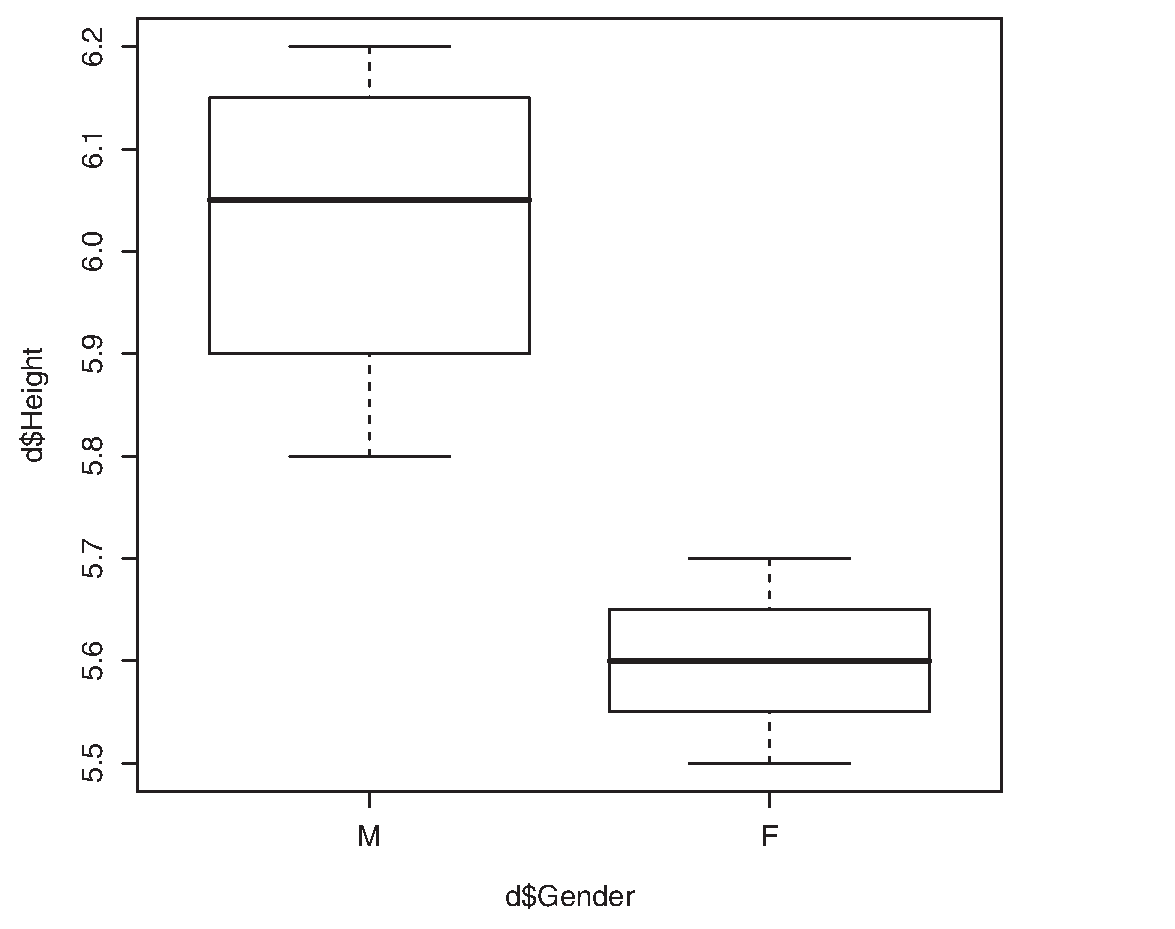
\includegraphics[width=0.65\textwidth]{img/rplot1}}
  \caption{A box plot, showing the distribution of heights by gender.}
  \label{fig:rplot1}
\end{figure}

Finally, let's take a look at R's plotting capabilities. First, we plot
the height ``as a function of'' the gender. (R uses the tilde
(\texttt{\~{}}) to separate control and response variables; the response
variable is always on the left.)

\begin{verbatim}
> plot( d$Height ~ d$Gender )
\end{verbatim}

This gives us a box plot, which is shown in Figure \ref{fig:rplot1}. 
On the other hand, if we plot the height as a function of the weight,
then we obtain a scatter plot (see Figure \ref{fig:rplot2}---without
the lines; we will add them in a moment).

\begin{verbatim}
> plot( d$Height ~ d$Weight, xlab="Weight", ylab="Height" )
\end{verbatim}

Given the shape of the data, we might want to fit a linear model to it.
This is trivially easy to do in R---it's a single line of code:

\begin{verbatim}
> m <- lm( d$Height ~ d$Weight )
\end{verbatim}

Notice once again the tilde notation used to indicate control and
response variable.

% dev.copy2eps( file="rplot2.eps", width=4, height=4 )
\begin{figure}[t!]
  \centerline{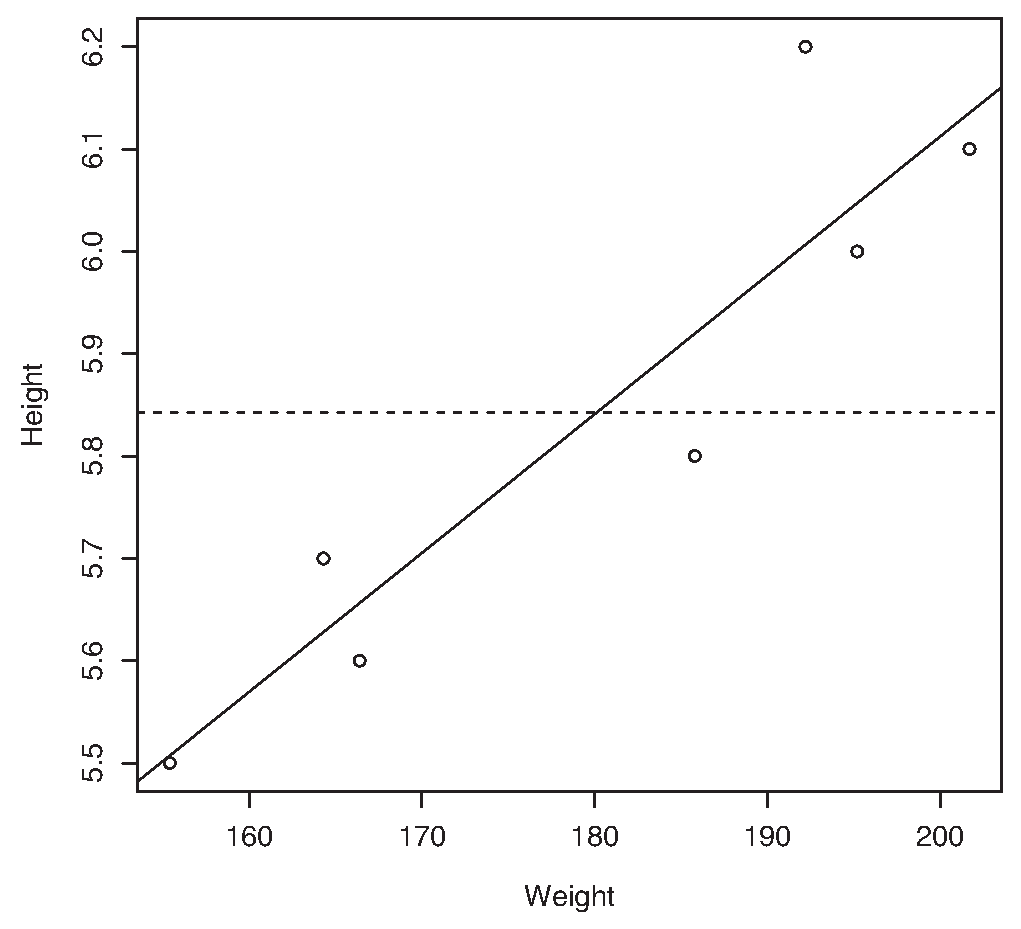
\includegraphics[width=0.65\textwidth]{img/rplot2}}
  \caption{A scatter plot with a linear fit.}
  \label{fig:rplot2}
\end{figure}

We may also want to add the linear model to the scatter plot with the
data. This can be done using the \texttt{abline()} function, which
plots a line given its offset (``a'') and slope (``b''). We can either
specify both parameters explicitly, or simply supply the result
\texttt{m} of the fitting procedure; the \texttt{abline} function can
use either. (The parameter \texttt{lty} selects the line type.)

\begin{verbatim}
> abline(m)
> abline( mean(d$Height), 0, lty=2 )
\end{verbatim}

This short example should have given you an idea of what working with
R is like.

R can be difficult to learn: it uses some unfamiliar idioms (such as
creative indexing) as well as some obscure function and parameter
names. But the greatest challenge to the newcomer (in my opinion) is
its indiscriminate use of function overloading. The same function can
behave quite differently depending on the (usually opaque) type of
inputs it is given. If the default choices made by R are good, then
this can be very convenient, but it can be hellish if you want to
exercise greater, manual control.

Look at our example again: the same \texttt{plot()} command generates
entirely different plot \emph{types} depending on whether the control
variable is categorical or numeric (box plot in the first case,
scatter plot in the latter).  For the experienced user, this kind of
implicit behavior is of course convenient, but for the beginner, the
apparent unpredictability can be very confusing. (In Chapter
\ref{ch:reduction}, we will see another example, where the same
\texttt{plot()} command generates yet a different type of plot.)

% The problem is that all these different plot types take different
% optional arguments (such as the \texttt{xlab}, \texttt{ylab} options
% used in the example), and it can be very difficult to predict which
% actual implementation of the generic \texttt{plot()} interface is
% being called at any given moment.

These kinds of issues do not matter much if you use R interactively
because you see the results immediately or, in the worst case, get an
error message so that you can try something else. However, they can be
unnerving if you approach R with the mindset of a contemporary
programmer who prefers for operations to be explicit. It can also be
difficult to find out which operations are available in a given
situation.  For instance, it is not at all obvious that the (opaque)
return type of the \texttt{lm()} function is admissible input to the
\texttt{abline()} function---it certainly doesn't look like the
explicit set of parameters used in the second call to
\texttt{abline()}.  Issues of this sort make it hard to predict what R
will do at any point, to develop a comprehensive understanding of its
capabilities, or how to achieve a desired effect in a specific
situation.

\index{statistics!R statistical analysis package|)} 
\index{R statistical analysis package|)}
\index{software!R statistical analysis package|)} 

% ============================================================
\section{Further Reading}

The number of introductory statistics texts seems almost
infinite---which makes it that much harder to find good ones. Below
are some texts that I have found useful:

\begin{itemize}
\item \cit{An Introduction to Mathematical Statistics and Its
    Applications}{Richard J.\ Larsen and Morris L.\ Marx}{4th ed.,
    Prentice Hall}{2005}
  This is my preferred introductory text for the mathematical
  background of classical statistics: how it all works. This is a math
  book; you won't learn how to \emph{do} practical statistical fieldwork from it. (It contains a large number of uncommonly interesting
  examples; however, on close inspection many of them exhibit serious
  flaws in their experimental design---at least as described in this
  book.) But as a mathematical treatment, it very neatly blends
  accessibility with sufficient depth.

\item \cit{Statistics for Technology: A Course in Applied
    Statistics}{Chris Chatfield}{3rd ed., Chapman \& Hall/CRC}{1983}
  This book is good companion to the book by Larsen and Marx.  It
  eschews most mathematical development and instead concentrates on
  the pragmatics of it, with an emphasis on engineering applications.

\item \cit{The Statistical Sleuth: A Course in Methods of Data
    Analysis}{Fred Ramsey and Daniel Schafer}{2nd ed., Duxbury
    Press}{2001}
  This advanced undergraduate textbook emphasizes the distinction
  between observational studies and controlled experiments more
  strongly than any other book I am aware of. After working through
  some of their examples, you will not be able to look at the
  description of a statistical study without immediately classifying
  it as observational or controlled (and questioning the conclusions
  if it was merely observational). Unfortunately, the development of
  the general theory gets a little lost in the detailed description of
  application concerns.

\item \cit{The Practice of Business Statistics}{David S.\ Moore,
    George P.\ McCabe, William M.\ Duckworth, and Layth Alwan}{2nd
    ed., Freeman}{2008}
  This is a ``for business'' version of a popular beginning
  undergraduate textbook. The coverage of topics is comprehensive, and
  the presentation is particularly easy to follow. This book can serve
  as a first course, but will probably not provide sufficient depth to
  develop proper understanding.


%\item \cit{The Practice of Business Statistics}{David S.\ Moore
%    et al}{2nd
%    ed., Freeman}{2008}
%  This is a ``for business'' version of a popular beginning
%  undergraduate textbook. The coverage of topics is comprehensive, and
%  the presentation is particularly easy to follow. This book can serve
%  as a first course but will probably not provide sufficient depth to
%  develop proper understanding.

\item \citnobreak{Problem Solving: A Statistician's Guide}{Chris
    Chatfield}{2nd ed., Chapman \& Hall/CRC}{1995}; and
  \cit{Statistical Rules of Thumb}{Gerald van Belle}{2nd ed.,
    Wiley}{2008}
  Two nice books with lots of practical advice on statistical fieldwork. Chatfield's book is more general; van Belle's contains much
  material specific to epidemiology and related applications.

\item \cit{All of Statistics: A Concise Course in Statistical
    Inference}{Larry Wasserman}{Springer}{2004}
  A thoroughly modern treatment of mathematical statistics, this book
  presents all kinds of fascinating and powerful topics that are
  sorely missing from the standard introductory curriculum. The
  treatment is advanced and very condensed, requiring general previous
  knowledge in basic statistics and a solid grounding in mathematical
  methods.

\item \cit{Bayesian Methods for Data Analysis}{Bradley P.\ Carlin,
    and Thomas A.\ Louis}{3rd ed., Chapman \& Hall}{2008}
  This is a book on Bayesian methods applied to data analysis problems
  (as opposed to Bayesian theory only). It is a thick book, and some
  of the topics are fairly advanced. However, the early chapters
  provide the best introduction to Bayesian methods that I am aware
  of.

% Can't use \pcit, because of the question mark at end of title
% \item \pcit{Sifting the Evidence---What's Wrong With Significance
%    Tests?}{Jonathan A.\ C.\ Sterne and George Davey Smith}{British
%    Medical Journal}{322}{2001}{226}\\

\item ``Sifting the Evidence---What's Wrong with Significance Tests?''
  Jonathan A.\ C.\ Sterne and George Davey Smith. \textit{British
    Medical Journal} 322 (2001), p.\ 226. \\
  This paper provides a penetrating and nonpartisan overview of the
  problems associated with classical hypothesis tests, with an
  emphasis on applications in medicine (although the conclusions are
  much more generally valid). The full text is freely available on the
  Web; a search will turn up multiple locations.
\end{itemize}




% Randomization 
% => establishes causal relationship
% 
% Replication
% => Reduces the variance (if measurement error is small and controlled)
% 
% Blocking
% => reduces experimental error (if we expect large, uncontrolled effects)
% 
% Factorial Experiment
% => interactions between 
% 
% 
% For all parametric tests: Normality assumption
%   Significant situations where violated: infinite second moment
%   (stock market, earth quakes - - - further examples?)
% 
% 
% Big Philosophical Difference: Domain knowledge - yes or no?
%   Physicists believe there to be a reliable and well-known process
%   generating the data.
%   Statisticians tend to ignore such knowledge - and are often trying
%   to answer questions for which it honestly does not exist: Twain letters
% 	
%   Also: Should data analysis lead to the formulation of justifiable
%   models, or not?
%   - Never believe an experiment that is not backed up by a good theory.
%   vs
%   - Don't use data that led to your hypothesis to test it.

\index{data analysis!statistics|)} 
\index{statistics|)} 


\clearpage

\thispagestyle{empty}

\cleardoublepage